
%% bare_conf.tex
%% V1.3
%% 2007/01/11
%% by Michael Shell
%% See:
%% http://www.michaelshell.org/
%% for current contact information.
%%
%% This is a skeleton file demonstrating the use of IEEEtran.cls
%% (requires IEEEtran.cls version 1.7 or later) with an IEEE conference paper.
%%
%% Support sites:
%% http://www.michaelshell.org/tex/ieeetran/
%% http://www.ctan.org/tex-archive/macros/latex/contrib/IEEEtran/
%% and
%% http://www.ieee.org/

%%*************************************************************************
%% Legal Notice:
%% This code is offered as-is without any warranty either expressed or
%% implied; without even the implied warranty of MERCHANTABILITY or
%% FITNESS FOR A PARTICULAR PURPOSE! 
%% User assumes all risk.
%% In no event shall IEEE or any contributor to this code be liable for
%% any damages or losses, including, but not limited to, incidental,
%% consequential, or any other damages, resulting from the use or misuse
%% of any information contained here.
%%
%% All comments are the opinions of their respective authors and are not
%% necessarily endorsed by the IEEE.
%%
%% This work is distributed under the LaTeX Project Public License (LPPL)
%% ( http://www.latex-project.org/ ) version 1.3, and may be freely used,
%% distributed and modified. A copy of the LPPL, version 1.3, is included
%% in the base LaTeX documentation of all distributions of LaTeX released
%% 2003/12/01 or later.
%% Retain all contribution notices and credits.
%% ** Modified files should be clearly indicated as such, including  **
%% ** renaming them and changing author support contact information. **
%%
%% File list of work: IEEEtran.cls, IEEEtran_HOWTO.pdf, bare_adv.tex,
%%                    bare_conf.tex, bare_jrnl.tex, bare_jrnl_compsoc.tex
%%*************************************************************************

% *** Authors should verify (and, if needed, correct) their LaTeX system  ***
% *** with the testflow diagnostic prior to trusting their LaTeX platform ***
% *** with production work. IEEE's font choices can trigger bugs that do  ***
% *** not appear when using other class files.                            ***
% The testflow support page is at:
% http://www.michaelshell.org/tex/testflow/



% Note that the a4paper option is mainly intended so that authors in
% countries using A4 can easily print to A4 and see how their papers will
% look in print - the typesetting of the document will not typically be
% affected with changes in paper size (but the bottom and side margins will).
% Use the testflow package mentioned above to verify correct handling of
% both paper sizes by the user's LaTeX system.
%
% Also note that the "draftcls" or "draftclsnofoot", not "draft", option
% should be used if it is desired that the figures are to be displayed in
% draft mode.
%
\documentclass[conference]{IEEEtran}
% Add the compsoc option for Computer Society conferences.
%
% If IEEEtran.cls has not been installed into the LaTeX system files,
% manually specify the path to it like:
% \documentclass[conference]{../sty/IEEEtran}





% Some very useful LaTeX packages include:
% (uncomment the ones you want to load)


% *** MISC UTILITY PACKAGES ***
%
%\usepackage{ifpdf}
% Heiko Oberdiek's ifpdf.sty is very useful if you need conditional
% compilation based on whether the output is pdf or dvi.
% usage:
% \ifpdf
%   % pdf code
% \else
%   % dvi code
% \fi
% The latest version of ifpdf.sty can be obtained from:
% http://www.ctan.org/tex-archive/macros/latex/contrib/oberdiek/
% Also, note that IEEEtran.cls V1.7 and later provides a builtin
% \ifCLASSINFOpdf conditional that works the same way.
% When switching from latex to pdflatex and vice-versa, the compiler may
% have to be run twice to clear warning/error messages.






% *** CITATION PACKAGES ***
%
%\usepackage{cite}
% cite.sty was written by Donald Arseneau
% V1.6 and later of IEEEtran pre-defines the format of the cite.sty package
% \cite{} output to follow that of IEEE. Loading the cite package will
% result in citation numbers being automatically sorted and properly
% "compressed/ranged". e.g., [1], [9], [2], [7], [5], [6] without using
% cite.sty will become [1], [2], [5]--[7], [9] using cite.sty. cite.sty's
% \cite will automatically add leading space, if needed. Use cite.sty's
% noadjust option (cite.sty V3.8 and later) if you want to turn this off.
% cite.sty is already installed on most LaTeX systems. Be sure and use
% version 4.0 (2003-05-27) and later if using hyperref.sty. cite.sty does
% not currently provide for hyperlinked citations.
% The latest version can be obtained at:
% http://www.ctan.org/tex-archive/macros/latex/contrib/cite/
% The documentation is contained in the cite.sty file itself.






% *** GRAPHICS RELATED PACKAGES ***
%
\ifCLASSINFOpdf
   \usepackage[pdftex]{graphicx}
  % declare the path(s) where your graphic files are
  % \graphicspath{{../pdf/}{../jpeg/}}
  % and their extensions so you won't have to specify these with
  % every instance of \includegraphics
  % \DeclareGraphicsExtensions{.pdf,.jpeg,.png}
\else
  % or other class option (dvipsone, dvipdf, if not using dvips). graphicx
  % will default to the driver specified in the system graphics.cfg if no
  % driver is specified.
   %\usepackage[dvips]{graphicx}
  % declare the path(s) where your graphic files are
  % \graphicspath{{../eps/}}
  % and their extensions so you won't have to specify these with
  % every instance of \includegraphics
  % \DeclareGraphicsExtensions{.eps}
\fi
% graphicx was written by David Carlisle and Sebastian Rahtz. It is
% required if you want graphics, photos, etc. graphicx.sty is already
% installed on most LaTeX systems. The latest version and documentation can
% be obtained at: 
% http://www.ctan.org/tex-archive/macros/latex/required/graphics/
% Another good source of documentation is "Using Imported Graphics in
% LaTeX2e" by Keith Reckdahl which can be found as epslatex.ps or
% epslatex.pdf at: http://www.ctan.org/tex-archive/info/
%
% latex, and pdflatex in dvi mode, support graphics in encapsulated
% postscript (.eps) format. pdflatex in pdf mode supports graphics
% in .pdf, .jpeg, .png and .mps (metapost) formats. Users should ensure
% that all non-photo figures use a vector format (.eps, .pdf, .mps) and
% not a bitmapped formats (.jpeg, .png). IEEE frowns on bitmapped formats
% which can result in "jaggedy"/blurry rendering of lines and letters as
% well as large increases in file sizes.
%
% You can find documentation about the pdfTeX application at:
% http://www.tug.org/applications/pdftex





% *** MATH PACKAGES ***
%
%\usepackage[cmex10]{amsmath}
% A popular package from the American Mathematical Society that provides
% many useful and powerful commands for dealing with mathematics. If using
% it, be sure to load this package with the cmex10 option to ensure that
% only type 1 fonts will utilized at all point sizes. Without this option,
% it is possible that some math symbols, particularly those within
% footnotes, will be rendered in bitmap form which will result in a
% document that can not be IEEE Xplore compliant!
%
% Also, note that the amsmath package sets \interdisplaylinepenalty to 10000
% thus preventing page breaks from occurring within multiline equations. Use:
%\interdisplaylinepenalty=2500
% after loading amsmath to restore such page breaks as IEEEtran.cls normally
% does. amsmath.sty is already installed on most LaTeX systems. The latest
% version and documentation can be obtained at:
% http://www.ctan.org/tex-archive/macros/latex/required/amslatex/math/





% *** SPECIALIZED LIST PACKAGES ***
%
%\usepackage{algorithmic}
% algorithmic.sty was written by Peter Williams and Rogerio Brito.
% This package provides an algorithmic environment fo describing algorithms.
% You can use the algorithmic environment in-text or within a figure
% environment to provide for a floating algorithm. Do NOT use the algorithm
% floating environment provided by algorithm.sty (by the same authors) or
% algorithm2e.sty (by Christophe Fiorio) as IEEE does not use dedicated
% algorithm float types and packages that provide these will not provide
% correct IEEE style captions. The latest version and documentation of
% algorithmic.sty can be obtained at:
% http://www.ctan.org/tex-archive/macros/latex/contrib/algorithms/
% There is also a support site at:
% http://algorithms.berlios.de/index.html
% Also of interest may be the (relatively newer and more customizable)
% algorithmicx.sty package by Szasz Janos:
% http://www.ctan.org/tex-archive/macros/latex/contrib/algorithmicx/




% *** ALIGNMENT PACKAGES ***
%
\usepackage{array}
% Frank Mittelbach's and David Carlisle's array.sty patches and improves
% the standard LaTeX2e array and tabular environments to provide better
% appearance and additional user controls. As the default LaTeX2e table
% generation code is lacking to the point of almost being broken with
% respect to the quality of the end results, all users are strongly
% advised to use an enhanced (at the very least that provided by array.sty)
% set of table tools. array.sty is already installed on most systems. The
% latest version and documentation can be obtained at:
% http://www.ctan.org/tex-archive/macros/latex/required/tools/


%\usepackage{mdwmath}
%\usepackage{mdwtab}
% Also highly recommended is Mark Wooding's extremely powerful MDW tools,
% especially mdwmath.sty and mdwtab.sty which are used to format equations
% and tables, respectively. The MDWtools set is already installed on most
% LaTeX systems. The lastest version and documentation is available at:
% http://www.ctan.org/tex-archive/macros/latex/contrib/mdwtools/


% IEEEtran contains the IEEEeqnarray family of commands that can be used to
% generate multiline equations as well as matrices, tables, etc., of high
% quality.


%\usepackage{eqparbox}
% Also of notable interest is Scott Pakin's eqparbox package for creating
% (automatically sized) equal width boxes - aka "natural width parboxes".
% Available at:
% http://www.ctan.org/tex-archive/macros/latex/contrib/eqparbox/





% *** SUBFIGURE PACKAGES ***
%\usepackage[tight,footnotesize]{subfigure}
% subfigure.sty was written by Steven Douglas Cochran. This package makes it
% easy to put subfigures in your figures. e.g., "Figure 1a and 1b". For IEEE
% work, it is a good idea to load it with the tight package option to reduce
% the amount of white space around the subfigures. subfigure.sty is already
% installed on most LaTeX systems. The latest version and documentation can
% be obtained at:
% http://www.ctan.org/tex-archive/obsolete/macros/latex/contrib/subfigure/
% subfigure.sty has been superceeded by subfig.sty.



%\usepackage[caption=false]{caption}
%\usepackage[font=footnotesize]{subfig}
% subfig.sty, also written by Steven Douglas Cochran, is the modern
% replacement for subfigure.sty. However, subfig.sty requires and
% automatically loads Axel Sommerfeldt's caption.sty which will override
% IEEEtran.cls handling of captions and this will result in nonIEEE style
% figure/table captions. To prevent this problem, be sure and preload
% caption.sty with its "caption=false" package option. This is will preserve
% IEEEtran.cls handing of captions. Version 1.3 (2005/06/28) and later 
% (recommended due to many improvements over 1.2) of subfig.sty supports
% the caption=false option directly:
%\usepackage[caption=false,font=footnotesize]{subfig}
%
% The latest version and documentation can be obtained at:
% http://www.ctan.org/tex-archive/macros/latex/contrib/subfig/
% The latest version and documentation of caption.sty can be obtained at:
% http://www.ctan.org/tex-archive/macros/latex/contrib/caption/




% *** FLOAT PACKAGES ***
%
%\usepackage{fixltx2e}
% fixltx2e, the successor to the earlier fix2col.sty, was written by
% Frank Mittelbach and David Carlisle. This package corrects a few problems
% in the LaTeX2e kernel, the most notable of which is that in current
% LaTeX2e releases, the ordering of single and double column floats is not
% guaranteed to be preserved. Thus, an unpatched LaTeX2e can allow a
% single column figure to be placed prior to an earlier double column
% figure. The latest version and documentation can be found at:
% http://www.ctan.org/tex-archive/macros/latex/base/



%\usepackage{stfloats}
% stfloats.sty was written by Sigitas Tolusis. This package gives LaTeX2e
% the ability to do double column floats at the bottom of the page as well
% as the top. (e.g., "\begin{figure*}[!b]" is not normally possible in
% LaTeX2e). It also provides a command:
%\fnbelowfloat
% to enable the placement of footnotes below bottom floats (the standard
% LaTeX2e kernel puts them above bottom floats). This is an invasive package
% which rewrites many portions of the LaTeX2e float routines. It may not work
% with other packages that modify the LaTeX2e float routines. The latest
% version and documentation can be obtained at:
% http://www.ctan.org/tex-archive/macros/latex/contrib/sttools/
% Documentation is contained in the stfloats.sty comments as well as in the
% presfull.pdf file. Do not use the stfloats baselinefloat ability as IEEE
% does not allow \baselineskip to stretch. Authors submitting work to the
% IEEE should note that IEEE rarely uses double column equations and
% that authors should try to avoid such use. Do not be tempted to use the
% cuted.sty or midfloat.sty packages (also by Sigitas Tolusis) as IEEE does
% not format its papers in such ways.





% *** PDF, URL AND HYPERLINK PACKAGES ***
%
%\usepackage{url}
% url.sty was written by Donald Arseneau. It provides better support for
% handling and breaking URLs. url.sty is already installed on most LaTeX
% systems. The latest version can be obtained at:
% http://www.ctan.org/tex-archive/macros/latex/contrib/misc/
% Read the url.sty source comments for usage information. Basically,
% \url{my_url_here}.





% *** Do not adjust lengths that control margins, column widths, etc. ***
% *** Do not use packages that alter fonts (such as pslatex).         ***
% There should be no need to do such things with IEEEtran.cls V1.6 and later.
% (Unless specifically asked to do so by the journal or conference you plan
% to submit to, of course. )


% correct bad hyphenation here
\hyphenation{op-tical net-works semi-conduc-tor}


\begin{document}
%
% paper title
% can use linebreaks \\ within to get better formatting as desired
\title{Energy Aggregation using Product of HMMs}


% author names and affiliations
% use a multiple column layout for up to three different
% affiliations
%\author{\IEEEauthorblockN{Michael Shell}
%\IEEEauthorblockA{School of Electrical and\\Computer Engineering\\
%Georgia Institute of Technology\\
%Atlanta, Georgia 30332--0250\\
%Email: http://www.michaelshell.org/contact.html}
%\and
%\IEEEauthorblockN{Homer Simpson}
%\IEEEauthorblockA{Twentieth Century Fox\\
%Springfield, USA\\
%Email: homer@thesimpsons.com}
%\and
%\IEEEauthorblockN{James Kirk\\ and Montgomery Scott}
%\IEEEauthorblockA{Starfleet Academy\\
%San Francisco, California 96678-2391\\
%Telephone: (800) 555--1212\\
%Fax: (888) 555--1212}}

% conference papers do not typically use \thanks and this command
% is locked out in conference mode. If really needed, such as for
% the acknowledgment of grants, issue a \IEEEoverridecommandlockouts
% after \documentclass

% for over three affiliations, or if they all won't fit within the width
% of the page, use this alternative format:
% 
%\author{\IEEEauthorblockN{Michael Shell\IEEEauthorrefmark{1},
%Homer Simpson\IEEEauthorrefmark{2},
%James Kirk\IEEEauthorrefmark{3}, 
%Montgomery Scott\IEEEauthorrefmark{3} and
%Eldon Tyrell\IEEEauthorrefmark{4}}
%\IEEEauthorblockA{\IEEEauthorrefmark{1}School of Electrical and Computer Engineering\\
%Georgia Institute of Technology,
%Atlanta, Georgia 30332--0250\\ Email: see http://www.michaelshell.org/contact.html}
%\IEEEauthorblockA{\IEEEauthorrefmark{2}Twentieth Century Fox, Springfield, USA\\
%Email: homer@thesimpsons.com}
%\IEEEauthorblockA{\IEEEauthorrefmark{3}Starfleet Academy, San Francisco, California 96678-2391\\
%Telephone: (800) 555--1212, Fax: (888) 555--1212}
%\IEEEauthorblockA{\IEEEauthorrefmark{4}Tyrell Inc., 123 Replicant Street, Los Angeles, California 90210--4321}}




% use for special paper notices
%\IEEEspecialpapernotice{(Invited Paper)}




% make the title area
\maketitle


\begin{abstract}
%\boldmath
The need to gather fine grained real-time spatio-temporal energy consumption data is fulfilled by the large scale deployment of smart meters. Remote monitoring on these meters is done by sending readings from the customer site to the data aggregators placed at the base stations. Each base station aggregates the load derived from all the meters connected to that station. The  readings received at the base station are adhoc and usually not synchronized in time. Each house is installed with multiple energy monitoring equipments such as smart meters and controllers. Different smart meters can send data points when they are collected resulting in inconsistent data including aggregating non-aligned time stamped readings, readings with missing values, repeated values, meter reset readings.
%The problem arises when the analytics is to be performed on the data which is aggregated from the inconsistent messages passed by all the meters connected to a particular base station.
%the demand response programs have been a cost effective alternative to meet the occasional peak demands. 
%We propose to solve the problem of energy aggregation where the constituents of each aggregate are inconsistent with respect to time. The challenges with the inconsistent data includes aggregating non-aligned time stamped readings, readings with missing values, repeated values, meter reset readings. 
We address the problem of learning from disparate data streams (with inconsistencies) by modelling streams as HMMs and the process of aggregating data at the base station as a Product of HMMs. This enables us to perform load forecasting using machine learning techniques. We have performed experiments using contrastive divergence learning on the Reference Energy Disaggregation Data Set (REDD) and the energy consumption data collected from the faculty housing at our institute. The results show that this technique performs the best by combining via product, all the HMMs (corresponding to each data stream) with binary states (on, off or standby) and training time linear to the number of HMMs.
%We address the problem of aggregating energy data in context with the load forecasting using a machine learning technique called product of Hidden Markov Models (PoHMM). 
%The objective function used for learning is the contrastive divergence between the observed data and the reconstructed data produced by running a Gibbs sampler. 
%Data analytics in energy domain, load forecasting on aggregates of power meters, Energy aggregation problem using pohmm, The STLF accuracy improves with larger aggregates, This paper deals with the energy aggregation problems in electrical system. The challenges included problem of aggregating inconsistent data, across time, in case of electrical systems.

\end{abstract}


% IEEEtran.cls defaults to using nonbold math in the Abstract.
% This preserves the distinction between vectors and scalars. However,
% if the conference you are submitting to favors bold math in the abstract,
% then you can use LaTeX's standard command \boldmath at the very start
% of the abstract to achieve this. Many IEEE journals/conferences frown on
% math in the abstract anyway.

% no keywords




% For peer review papers, you can put extra information on the cover
% page as needed:
% \ifCLASSOPTIONpeerreview
% \begin{center} \bfseries EDICS Category: 3-BBND \end{center}
% \fi
%
% For peerreview papers, this IEEEtran command inserts a page break and
% creates the second title. It will be ignored for other modes.
\IEEEpeerreviewmaketitle



\section{Introduction}
% no \IEEEPARstart
Smart meters consisting of real time sensors, power outage notifications and power quality monitoring are widely used today. These meters provide a host of benefits like energy efficiency and savings, improved retail competition, better demand response actions, improved tariffs, lower bills due to better customer feedback, accurate billing, less environmental pollution, etc. \cite{Klopfert}
They generate huge amount of time series data which can be used for gaining meaningful insights through analytics.
They can measure site specific information and also help agencies set different electricity prices for consumption based on the time of the day, seasons, holidays, etc. Based on the data collected from smart meters, a feedback sent to the customers by the utilities that can help consumers better manage their resources. A research \cite{mckerracher} shows that by providing real time feedback, consumers can reduce the consumption by 3-5\%.
%This helps consumers to better manage their energy resources and reduce their bills and carbon emissions.


In recent years, machine learning has been applied to the problem of energy consumption and demand forecasting analysis. The role of the machine learning algorithm is to study the sensor data and provide alerts and warnings when anomalous behaviour occurs or to inform (and remind) customers when certain activities were performed, which rooms they occupied, and what appliances they used most frequently during that period. This information can be transmitted to customers in timely fashion via phone, email or the Internet.
Chicco et al. \cite{1626400} compared several clustering techniques and observed that the hierarchical clustering and modified follow-the-leader perform best among the rest K-Means, fuzzy K-Means to group customers with similar electrical behaviour \cite{5620917}. Another paper \cite{Wijaya} used classifiers like random forest, decision trees (J48), logistic and naive bayes to identify customers with similar electricity consumption profiles.
%Sensor data collected from smart homes are used to reveal activity patterns of the residents, which can then be correlated with the total energy consumption. This enables utility companies and their customers to associate activities with energy usage and costs, devise intelligent systems to control home environments improving energy efficiency and reducing costs. Typically, sequences of usage patterns that appear frequently at different time scales (daily, weekly, monthly, yearly) and across different homes are studied and 
%%; trends of electricity consumption (steadily increasing, decreasing, cyclic, seasonal) for individual homes and across the community; and anomalies (sudden peaks or drops on consumption) for individual homes and across the community.
%outlier detection algorithms are designed to enable customers to be notified that they are consuming unusually large amount(s) of energy during some specific period. 
Related problems involve study of trends of electricity consumption (steadily increasing, decreasing, cyclic, seasonal) and sudden anomalous behaviour (sudden peaks or drops on consumption) for individual homes and across the community.\cite{Diane}

In this paper, we use Hidden Markov models (HMMs) to analyse the time series energy data. HMMs are widely used for time series data like financial time series prediction \cite{SS97a}, health checkup data \cite{Kawamoto}, energy time series analytics \cite{Albert}, etc.\\
We model the data stream from each source as a HMM with its states represented as ON/OF.  For $N$ sources, there are $N$ HMMs and  the total number of states collectively are $2^N$. The observations represent the energy consumed in a particular state. These observations are recorded at different time scales for different sources. \\
In order to aggregate the data from all the different sources, we build a machine learning model using products of HMMs (PoHMMs) and apply it to the energy aggregation problem. There are many reasons why the product model constructed from many HMMs is appropriate. 
%First, this model is ideal for data which is caused by multiple underlying influences.
%First, this model allows each HMM to make decisions based on few dimensions without actually having to worry about covering the full dimensionality of the problem.
First, in a high-dimensional space each model constrains a different subset of dimensions, and their product constrains all of the dimensions.
Second, HMMs alone are not efficient at capturing long range structure in time series \cite{Taylor} -- in contrast to PoHMMs  \cite{andrew} allow each model to remember a different piece of information about the past.
Two different proof of concepts are presented -- first one on the REDD \footnote{http://redd.csail.mit.edu/} data set and the other one on real data collected at the faculty housing in India. 
%application of are aggregating energy consumption information using a model that extends the power of HMMs. HMM's are used as the basic expert in the of product of experts model. 

%There have been some experiments on sentence and character strings modelling, factorial time series to demonstrate the advantages of using a PoHMM over an equivalently sized regular HMM}.
%We have applied the contrastive divergence learning algorithm on two datasets, REDD dataset and the faculty housing dataset which was generated by smart meters.
%The system architecture for the faculty housing dataset consists of two smart meters $S_1$ and $S_2$ installed in a faculty housing building collecting data from twelve floors. $S_1$ collects data from first six floors (0 to 5th) and $S_2$ collects data from the rest of the floors (6 to 11th). The data collected from two meters is aggregated using product of experts technique in a way that the contrastive divergence between the two probability distributions is minimized. 
%The proof of concept of REDD dataset and faculty housing dataset is given in section~\ref{sec:redd} and section~\ref{sec:faculty} respectively.

\noindent \textbf{Organization:} This paper is organized as follows: Section~\ref{related} examines related work on data analytics on aggregated data of smart meters; Section~\ref{sec:review} provides a review of products of Hidden Markov Models (HMMs) and how they relate to our application. The two proofs of concepts are introduced in Section~\ref{poc} and Section~\ref{poc2} to illustrate the effectiveness of the use of product of HMMs in the energy aggregation problem. Finally, Section~\ref{con} concludes the work.


\section{Related Work}
\label{related}
In this section, we describe work that uses ensemble learning techniques and non-ensemble learning techniques to solve problems in energy domain.
\subsection{Non-ensemble based learning techniques}

\subsubsection{Energy Aggregation}
%Devaine et al. (CITE) study ...
In wireless sensor networks, energy data aggregation is a method of combining data from different sources and expressing on a specific variable, in a summarised format. As the sensor network generates lot of data for the end user to process, there are automated methods employed to aggregate data. This data fusion is generally known as data aggregation which combines the data into a set of meaningful information \cite{Heinzelman00energy}.
The sensor nodes are organised in a tree structure, called aggregation tree. The leaves of this tree are the sensor devices, the internal nodes are the aggregator devices that takes the data from the leaves, aggregates it and sends it to its parent node which is the root of the tree. \\
The main objective of data aggregation is to reduce the unnecessary information thereby reducing the network traffic and improving the privacy of the customers from internal and external entities by keeping only the necessary information \cite{taban}. 


%To study the process of energy aggregation, data is collected from multiple smart meters. This collected data is very large which in turn makes the analytics on top of it very difficult. Also, this detailed energy consumption data leads to privacy breach and other risks related to it. To address this problem, there has been work done \cite{Wijaya} to reduce the smart meter data numerosity by converting it into symbolic representation and then allowing algorithms on top of it. They have applied the symbolic representation tasks for customer segmentation and load forecasting.

%The purpose of energy aggregation is to get some valuable information about single or multi-site units. 
%This work evaluates the trend of degrading performance of the state of the art algorithms when the number of considered meters decrease \cite{BLTJ:BLTJ21650}. Short term load forecasts at the meter level help the company communicate with the customer about energy savings and billing. STLF handles prediction of one hour upto one week.
%The energy aggregation problem has been tackled in a variety of ways including topology control, energy conserving sleep scheduling, mobile data collectors and data aggregation. 
%Research has been done on the role of energy on the growth of the country's economy \cite{NYAS:NYAS5921}.

\subsubsection{Energy Disaggregation}
The process in which the whole building energy (aggregated) signal is separated into appliance level energy (disaggregated) for a variety of reasons like residential energy reductions, program evaluation, targeted marketing, etc. Several studies have been done in this regard, one of the unsupervised desegregation method \cite{DisaggregationHSMM} that outperforms other unsupervised disaggregation methods is conditional factorial hidden semi-Markov model. This model when integrated with other features, accurately represents the individual appliance energy consumption. Another research \cite{KolterJ12} that exploits the additive structure of the FHMM to develop approximate inference procedure in  energy disaggregation domain that outperforms the rest.

\subsubsection{Load Forecasting}
Electrical load forecasting refers to the projection of electrical load required in a certain geographical area with the use of previous electrical load usage in the same area. It is extremely important for efficient power system planning and operation, energy purchasing and generation, load switching, infrastructure development. It encompasses various factors like, historical load, weather data, population, energy supply and price, time of the year, etc.
It is usually divided into three categories, short-term forecasts (one hour to one week) , medium-term forecasts (one week to one year) and long-term forecasts (more than a year).
In short term load forecast, \cite{Bakirtzis} and \cite{Chen} used a three layer feed forward artificial neural network and to predict daily load profiles. In a paper by \cite{Chow}, nonlinear autoregressive integrated neural network was used to predict daily load consumption.
In medium term load forecasts, the author forecasts \cite{Falvo} the monthly load through knowledge based activities from the output of the ANN based stage providing yearly energy predictions. Whereas in \cite{bassi}, time lagged feedforward neural network is used to do monthly forecasting on the basis of historical series of electrical load, economic and demographic variables. And the authors from covenant university, \cite{samuel} performed load forecasting of their own educational institute using the models based on linear, compound growth and cubic methods of regression analysis.
In long term load forecasting, study done by \cite{Daneshi} resulted in showing that the models based on regression analysis did not give very accurate predictions as compared to fuzzy neural network which performed better due to better handling with non linear systems. Another work  \cite{Zhang} uses support vector regression to derive non linear relationship between load and economic factors like GDP for long term forecasting in developing countries.



\subsubsection{Customer Segmentation}
The identification of consumer profiles that show similar behaviour in energy consumption. This analysis is useful in various ways, like demand response system, intelligent distribution channel. The author \cite{wijaya2014consumer} segments the customers based on contextual dimensions like location, seasons, weather patterns, holidays, etc which help with various higher level applications like usage-specific tariff structure, theft detection, etc. In \cite{Albert}, author proposes to infer occupancy states from consumption time series data by using HMM framework. They investigate the effectiveness of HMM and model based cluster analysis in producing meaningful features of the classification. This work suggests the dynamics of time series as captured by HMM analysis can be valuable.

\subsection{Ensemble based learning techniques}
Ensemble learning is a method where multiple learners are trained to solve the same problem. It constructs a set of hypothesis and combines them to generate the final result.
\subsubsection{Prediction with expert advice}
A study done by \cite{Shen}, proposed a Pattern Forecasting Ensemble Model (PFEM) comprising of five forecasting models using different clustering techniques, like k-means model, self-organising map model, hierarchical clustering model, k-medoids model and fuzzy c-means model. They have showed that on three real-world dataset, their proposed ensemble model outperformed all the five individual model in case of day ahead electricity demand prediction.
Another study \cite{Felice} highlighted the importance of regularised negative correlation learning ensemble methodology on the problem of energy load hourly prediction. This method tried to overcome the problem of variability in neural network due to high sensitivitiness to the initial conditions. As this method combines the outputs of several neural networks, it achieves a marked reduction in error after introducing external data. \\
An extension of HMMs, called Factorial Hidden Markov Model (FHMM) \cite{fhmm} is a class of ensemble based learning models that addresses the need for distributed hidden states in HMMs. But by being a directed model, when conditioned on the observed sequence, the hidden state chains become independent making the inference easy but learning more complex. But this approach has proved to be very inefficient in high dimensional spaces.
To model a complicated, high-dimensional data distributions, an approach called mixture of gaussians is widely used. In this method, each simple model which is a gaussian is combined using a weighted arithmetic mean of individual distributions. Such mixtures of tractable models can easily fit to data using expectation-maximization (EM) and are more powerful than their individual component. So, a different way of combining these distributions is by multiplying them together and then renormalizing them.
In our paper,  we deal with the problem of energy aggregation using ensemble learning model. Each HMM is used to represent a state of an appliance. An appliance can have states like ON or OFF. The combination of the outputs from each of these HMM models gives us our ensemble based learning model, Product of Hidden Markov Model (PoHMM) \cite{hinton2000}. This learning technique outputs the probability distribution by combining the outputs from several simpler distributions. It allows each model to make a decision on the basis of few dimensions.




\begin{figure*}
\centering
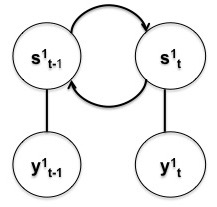
\includegraphics[width=4cm,height=3cm]{hmm1.jpg}
\label{fig:hmm1}
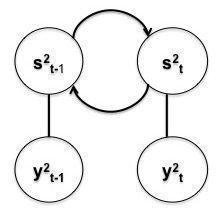
\includegraphics[width=4cm,height=3cm]{hmm2.jpg}
\label{fig:hmm2}
\caption{HMM $S^1$ and $S^2$}
\end{figure*}


\section{Review}
\label{sec:review}

%Benveniste defines HMM as a triple (\'{A}, $\mu$, $\pi$) where \'{A} = (X,$X_0$,A,T) is an automaton, $\mu$ is the initial state probability, $\pi$ is factored as state transition probability $\pi$$_{x}$ and message transition probability $\pi$$_{A}$. He uses a random arbiter $\alpha$, with values {first, second, third} to choose automaton to initiate transition. If $\alpha$ = first then first automaton chooses any transition having a private message whereas second automaton performs a stuttering transition, and vice versa for $\alpha$ = second. If $\alpha$ = both, then both automata agree on some shared message and move accordingly.

A Hidden Markov Model (HMM) is a statistical markov model that represents the probability distribution over a sequence of observations \cite{Ghahramani}. They are found useful in applications like speech \cite{Rabiner}, handwriting, gesture recognition, part-of-speech tagging, bioinformatics, etc. It has two properties, first, the observation at time $t$, $y_{t}$ is generated by a process whose state at time $t$, $s_{t}$ is hidden from the observer and second, is that this hidden state process satisfies markov property which states that given the value at state $s_{t-1}$, the value at current state $s_{t}$ is independent of all the states prior to $t-1$. The subscripts $i$ and superscripts $j$ indicate the model at $i$th time and the $j$th HMM. The state space of the HMM is discrete, that is a state can take $2$ values denoted by ON and OFF. The observed values represent the aggregated load/energy collected from different data streams at time $t$. In order to define probability distribution over the sequence of observation, it is important to define probability distribution over the initial state P($s_{1}$), the transition probability P($s_{t}|s_{t-1}$) and the observed probability P($y_{t}|s_{t}$) where $y_{t}$ is the observation at time $t$. \\
Following a notation in \cite{Rabiner}, HMM is composed of a 3-tuple \{A, B, $\pi$ \} where A is the transition probability, B is the observed probability and $\pi$ is the initial state probability.
%HMMs are widely used for modelling time series data. They are found useful in applications like speech, handwriting, gesture recognition, part-of-speech tagging, bioinformatics, etc.
HMMs solve three fundamental problems:
1. Given the model $\lambda$ = \{A, B, $\pi$ \}, and observation sequence Y = \{$y_{1}$,...,$y_{T}$\}, how do we efficiently compute the probability of the sequence of observations given the model, that is P($Y|\lambda$).
2. Given the model $\lambda$ and observation sequence Y, what is the underlying state sequence \{$s_{1}$,...,$s_{T}$\} that best explains the observations.
3. Given the observation Y and state space sequence S, how do we need to adjust the parameters so as to find the model $\lambda$ that maximises P($Y|\lambda$).\\
In this paper, we deal with the third problem as it involves learning parameters by training the model with the historical data and then using these parameters to predict the future observations.
The figure ~\ref{fig:hmm1} shows the HMM $S^1$ and $S^2$ generated by a data stream.

%Using the traditional HMM notation for the parameter $\lambda$ = \{A, B, $\pi$ \} where A is the transition probability, B is the observed probability and $\pi$ is the initial state probability. For HMMs, $S^{1}$ \& $S^{2}$ we have the values of A, B, $\pi$ as shown in table ~\ref{table:A}, ~\ref{table:B}, ~\ref{table:pi} respectively.

%Distributed networks can be modeled using interacting automata.
%Benveniste \cite{benveniste} defines automaton as a quadruple, \'{A} = (X,$X_0$,A,T) where X is a finite state of sets, $X_0$ is the subset of initial states, A is a finite set of messages, T is a set of transitions of the form t = \{x\_,a,x\} where x\_ is the previous state, a is the message label on which the state transitions to the next state x. The figure~\ref{fig:ex} below explains the automata with an example.\\


%For HMM R, X$_{R}$ = \{2; $R_1$,$R_2$\}, X$_{0R}$ = \{$R_1$\}, A$_{R}$ = \{a,b\}, T$_{R}$ = \{$R_1$,a,$R_1$; $R_1$,b,$R_2$; $R_2$,a,$R_2$; $R_2$,b,$R_1$\} \\
%For HMM S, X$_{S}$ = \{3; $S_1$,$S_2$,$S_3$\}, X$_{0S}$ = \{$S_1$\}, A$_{S}$ = \{a,b\}, T$_{S}$ = \{$S_1$,a,$S_1$; $S_1$,b,$S_2$; $S_2$,a,$S_2$; $S_2$,b,$S_3$; $S_3$,a,$S_3$; $S_3$,b,$S_1$\} \\
%The product of two HMMs P = R x S is defined as follows: \\
%X = X$_{R}$ x X$_{S}$ \\
%$X_0$ = X$_{0R}$ x X$_{0S}$ \\
%A = A$_{R}$ $\cup$ A$_{S}$ \\
%t = (x\_,a,x)  \\

%Benveniste uses a notion of stuttering transition which helps to distinguish between local and global time by inserting dummy transitions between two transitions of a local automaton attached to a node. This stuttering transition waits for others to progress.

%\begin{table}[h]
%\centering
%\begin{tabular}{ l | c | c }
% $A_{S^{1}}$ & $S^1_1$ & $S^1_2$ \\
%\hline
%$R_1$ & 0.6 & 0.4 \\
%$R_2$ & 0.3 & 0.7 \\
%\end{tabular}
%\quad
%\begin{tabular}{ l | c | c | c }
%  $A_{S^{2}}$ & $S^2_1$ & $S^2_2$ & $S^2_3$ \\
%\hline
%$S_1$ & 0.6 & 0.3 & 0.1 \\
%$S_2$ & 0.4 & 0.1 & 0.5 \\
%$S_3$ & 0.2 & 0.4 & 0.4 \\
%\end{tabular}
%\caption{Transition probabilities, A}
%\label{table:A}
%\end{table}
%
%\begin{table}[h]
%\centering
%\begin{tabular}{ l | c | c }
% $B_{S^{1}}$ & a & b \\
%\hline
%$S^1_1$ & 0.2 & 0.8 \\
%$S^1_2$ & 0.5 & 0.5 \\
%\end{tabular}
%\quad
%\begin{tabular}{ l | c | c | c}
% $B_{S^{2}}$ & a & b & c\\
%\hline
%$S^2_1$ & 0.2 & 0.3 & 0.5 \\
%$S^2_2$ & 0.5 & 0.4 & 0.1 \\
%$S^2_3$ & 0.4 & 0.3 & 0.3 \\
%\end{tabular}
%\caption{Observed probabilities, B}
%\label{table:B}
%\end{table}
%
%\begin{table}[h]
%\centering
%\begin{tabular}{ l | c | c }
%&  $R_1$ & $R_2$ \\
%\hline
%$\pi_{S^{1}}$ & 0.4 & 0.6 \\
%\end{tabular}
%\quad
%\begin{tabular}{ l | c | c | c}
%&  $S_1$ & $S_2$ & $S_3$\\
%\hline
%$\pi_{S^{2}}$ & 0.4 & 0.4 & 0.2 \\
%\end{tabular}
%\caption{Initial state probabilities, $\pi$}
%\label{table:pi}
%\end{table}

%Talking in terms of HMM, requires us to equip products of automata with probabilities. 

\subsection{Product of HMMs}
\label {sec:pohmm}
PoHMM is a model that combines several HMMs by multiplying their individual distribution together and then renormalizing them. Its representation includes both directed and undirected links where the hidden states are causally connected to the other hidden states but non causally related to the visible states. This causes different conditional independence relationships among the variables in graphical model. 
%It is a way of combining HMM's to form distributed state time series model. It is defined by multiplying together the densities of its, k experts and renormalizing them. 
The figure~\ref{fig:product} is a product of two HMMs P = $S^1$ x $S^2$ where the superscript in $S^1$ indicates the kth HMM. The number of states in the PoHMM is the product of states in $S^1$ and $S^2$ which is $4$ in our case. The connections formed in the P depend on the links in the multiplying HMMs. 
%The resultant HMM will have a pair (s,s) X = \{6; $R_1$$S_1$, $R_1$$S_2$, $R_1$$S_3$, $R_2$$S_1$, $R_2$$S_2$, $R_2$$S_3$\} \\
%$X_0$ = \{$R_1$$S_1$\} \\
%A = \{a,b\} \\


%The rules for synchronised product construction are : \\
%1. $<p,q>$ --a--$>$ $<p',q>$ if a $\in$ A$_{R}$ $\cap$ A$_{S}$ and p --a--$>$ p' and q --a--$>$ q'	\\
%2. $<p,q>$ --a--$>$ $<p',q>$ if a $\in$ A$_{R}$, a $\notin$ A$_{S}$ and p --a--$>$ p'	\\
%3. $<p,q>$ --a--$>$ $<p,q'>$ if a $\notin$ A$_{R}$, a $\in$ A$_{S}$ and q --a--$>$ q'	\\

 \begin{figure*}[!t]
\centering
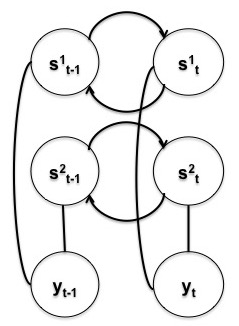
\includegraphics[width=4cm,height=4cm]{product}
\caption{Product of HMMs, P = $S^{1}$ x $S^2$}
\label{fig:product}
\end{figure*}


\subsection{Training the model by minimising contrastive divergence}
%Product of experts (PoE)\footnote{http://en.wikipedia.org/wiki/Product\_of\_experts} is a technique that models probability distribution by combining the output from several simpler distributions. It is defined by the following formula:\\
% Write the formula and explain it. Explain Gibbs Sampling

To fit the model to the data, we need to maximize the likelihood of the dataset or minimise the Kullback-Liebler divergence between the data distribution, $P^0$ (data distribution at time 0) and the equilibrium distribution over the visible variables, $P^\infty_\theta$ (fantasy data) which is obtained after prolonged Gibbs sampling as shown in equation~\ref{eq:KL}. 

\begin{eqnarray}
P^0 || P^\infty_\theta = \sum_{d}P^0 (d)logP^0(d) - \sum_{d}P^0 (d)logP^\infty_\theta(d) \label{eq:KL} \\
P^0 || P^\infty_\theta = -H(P^0) - \langle log P^\infty_\theta \rangle_{P^{0}}
\end{eqnarray}

where $||$ represents Kullback-Leibler divergence, d is the data vector in discrete space, $\theta_m$ is all the parameters of individual model m, $P^0$ is the data distribution at time $0$, H($P^0$) represents the entropy which is ignored during optimisation as $P^0$ does not depend on the parameters of the model, angle brackets denote the expectation over the distribution specified by the subscript.
In Gibbs sampling, each variable draws a sample from its posterior distribution given the current states of the other variables. The hidden states of all the models are conditionally independent given the data and hence can be parallel updated as shown in Figure~\ref{fig:gibbs}. At time t=0, the observed variables represent a data vector, d and the hidden variables, s of all the models are updated in parallel with samples from their posterior distribution given the observed variables, y. At time 1, the visible variables are updated to generate a reconstruction of the original data vector from the hidden variables and the hidden variables are again updated simultaneously. This prolonged sampling helps the Markov chain to converge to the equilibrium distribution which helps to attain the unbiased estimate of the gradient of the PoHMMs. But since the samples from the equilibrium state have high variance as they come from the entire model's distribution, it poses a difficulty in determining the estimate the derivative. Therefore, the optimisation is performed on the different objective function called contrastive divergence, defined in equation~\ref{eq:CD}. Contrastive divergence is the difference between $P^0 || P^\infty_\theta$ and $P^1_\theta || P^\infty_\theta$ where $P^1_\theta$ is the distribution over the one-step reconstruction of the data vectors generated by one full step of Gibbs sampling. The intuition behind using contrastive divergence is to leave the initial distribution $P^{0}$ over the visible variables unaltered and also the intractable expectation over $P^\infty_\theta$ gets cancelled out. Instead of comparing the initial and final derivatives, $P^0$ and $P^\infty_\theta$, the Markov chain is run for one full step and the parameters are updated to avoid the chain to wander away from the initial distribution on the first step. As $P^1$ is a step closer to $P^\infty$ which guarantees that $P^0 || P^\infty_\theta$ will always exceed $P^1_\theta || P^\infty_\theta$ ensuring a non negative value unless $P^0$ = $P^1_\theta$. If $P^0$ = $P^1_\theta$, then it implies that the chain is already in an equilibrium state, that is $P^0$ = $P^\infty_\theta$ hence making the value of contrastive divergence as $0$.

 \begin{figure*}[t]
\centering
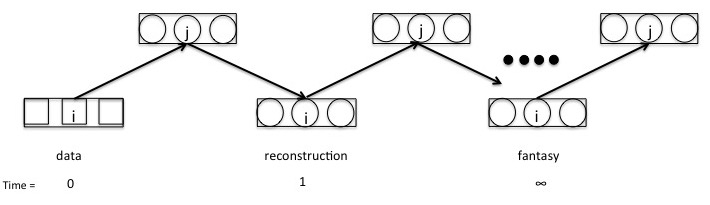
\includegraphics[width=12cm,height=4cm]{gibbs.jpg}
\caption{Visualization of Gibbs sampling}
\label{fig:gibbs}
\end{figure*}

\begin{eqnarray}
- \frac {\partial} {\partial\theta_{m}} (P^0 || P^\infty_\theta - P^1_\theta || P^\infty_\theta) = \langle \frac {\partial log f_{\theta_{m}}}{\partial \theta_m} \rangle_{P^0} \\
- \langle \frac {\partial log f_{\theta_{m}}}{\partial \theta_m} \rangle_{P^1_\theta} + \nonumber \frac{\partial{P^1_\theta}}{\partial\theta_m} \frac{\partial(P^1_\theta || P^\infty_\theta)}{\partial{P^1_\theta}}
 \label{eq:CD}
\end{eqnarray}
where log$f_{\theta_{m}}$ is a random variable that can also be written as $f_m$($D|\theta_m$) where D being a random variable corresponding to the data.
In equation~\ref{eq:CD}, the first two terms on the right hand side are tractable as it is easy to sample from $P^0$ and $P^1_\theta$ but the third term represents the effect on $P^1_\theta || P^\infty_\theta$ of the change of the step reconstruction caused by the change in the $\theta_m$. Extensive simulations show that it is small and rarely differs from the result of other two terms, hence can be safely ignored. Therefore in contrastive divergence, the parameters are learned according to the equation~\ref{eq:params}. To minimise the contrastive divergence by using a Markov chain that slowly mixes, we can use mixing techniques like weight decay that ensures that every possible visible vector has non zero probability given the latent variables.

\begin{eqnarray}
\Delta\theta_m \propto \langle \frac {\partial log f_{\theta_{m}}}{\partial \theta_m}\rangle_{P^0} - \langle \frac {\partial log f_{\theta_{m}}}{\partial \theta_m} \rangle_{P^1_\theta} \label{eq:params}
\end{eqnarray}

The contrastive divergence algorithm for training the PoHMM has the following steps:
\begin{enumerate}
\item Each model's gradient $\frac{\partial}{\partial\theta_m}$ $P(Y|\theta_m)$ ($\{y_t\}_{t=1}^T$ = Y is the visible variable) is calculated on a data point using forward backward algorithm.
\item A sample for each model is taken from the posterior distribution of paths through state space.
\item At each time step, the distributions are multiplied and renormalized together to get the reconstruction distribution.
\item A sample from the reconstruction distribution is drawn at each time step to get a reconstructed sequence. Each model's is gradient is computed on the new sequence $P(\hat Y|\theta_m)$
\item Parameters are updated as per equation~\ref{eq:params}

\end{enumerate}
%High dimensional distributions are approximated as a product of one dimensional distributions. The product of individual distributions which are uniguassian or multivariate guassian will also be multivariate guassian. If the individual models are more complicated and contain one or more hidden variables, multiplying their distributions together and renormalizing them can be very powerful. These individual models are called "experts".
%The product of experts produce sharper distribution than the individual distributions\cite{hinton2000}.

\subsection{Inference in PoHMM}

The main feature of PoHMMs is its undirected graphical modelling with no direct connection among the latent variables ($S^1_{t}$ and $S^2_{t}$) as they only interact indirectly via observed variables ($Y_{t}$). The hidden variables all the experts are rendered independent when conditioned on visible variables. So, if the inference in each of the constituent model is tractable then the inference in the product is also tractable. To generate a data point in this model, all the models in PoHMMs generate an observation and if they all generated the same point then it is accepted else they again generate an observation until all the models agree to it. Therefore all the models have some influence over the generated data. So, the inference determines the the probability that all the models would have taken in order to generate the given observation. 

%\begin{figure*}[t]
%\centering
%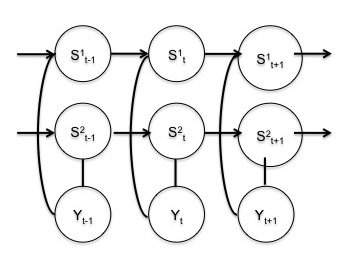
\includegraphics[width=5cm,height=3cm]{pohmm1.jpg}
%\caption{Product of HMMs, P = $S^{1}$ x $S^2$}
%\label{fig:PoHMM}
%\end{figure*}

\section{Applications using Product of HMM}
\label{poc}

\textbf{Aim}: To perform load forecasting using PoHMMs.
%To represent streams of energy consumption data from $n$\footnote{n=2} appliances by product of $k$ HMMs.

\subsection{Data Description} 
\begin{itemize}
\item \textbf{Dataset 1:} The Reference Energy Disaggregation Data Set (REDD) contains power consumption data from real homes, for the whole house as well as for each individual circuit in
the house (labeled by the main type of appliance on that circuit). %It is intended for use in developing disaggregation methods, which can predict, from only the whole-home signal, which devices are being used.
The REDD data set contains two main types of home electricity data: high-frequency current/voltage waveform data of the two power mains (as well as the voltage signal for a single phase), and lower-frequency power data including the mains and individual, labeled circuits in the house. 
The main directory consists of several house directories, each of which contain all the power readings for a single house.  Each house subdirectory consists of a labels and channels files. The labels file helps in matching the channel number with the device name. Each channel file has two columns containing UTC timestamps (as integers) and power readings (recording the apparent power of the circuit) for the channel.
Experiments reported here use the house 2 data from REDD. The dataset has $318759$ records and $2$ columns. We randomly sample $300$ records for our initial experiment.
%The time series data of the microwave, dryer, kitchen$\_2$ and refrigerator are plotted below in Figures~\ref{fig:micro}, ~\ref{fig:washer}, ~\ref{fig:kitchen2}, ~\ref{fig:refri}. 
The implementation of the product of hidden markov model is obtained from Iain Murray's website\footnote{\label{link}http://homepages.inf.ed.ac.uk/imurray2/code/}. It implements the technique described in Geoff Hinton's paper \cite{hinton2000}.
%Time series data from two appliances are represented as product of $k$ HMMs. It has $11$ channels where each channel corresponds to the following appliance, 1. mains1, 2. mains2, 3. kitchen 1, 4. lighting, 5. stove, 6. microwave, 7. washer dryer, 8. kitchen 2, 9. refrigerator, 10. dishwasher, 11. disposal


\item \textbf{Dataset 2:} This data represents the energy consumed by the institue's faculty housing building. As a part of research, a team from the institue has installed various temperature, light and motion sensors to perform real world studies and to analyse user preferences for energy conservation. For our analysis, we selected $1$ month's historical data ranging from 01-01-2014, 00:01 hours to 31-01-2014, 23:59 hours. The two smart meters installed captures the data from all the $12$ floors. The first meter records readings from ground to $5$th floors and the second meter from $6$th to $11$th. The dataset includes timestamp and power consumed in watts. There are $84133$ records in this dataset. We also have the total energy consumed by the faculty housing building which would serve as the ground truth to compare the aggregated load using PoHMMs. The data is obtained from the website whose screenshot is shown in Figure~\ref{fig:screenshot}
%Time series data from two streams are modelled as a product of $k$ HMMs. 


\begin{figure*}[t]
\centering
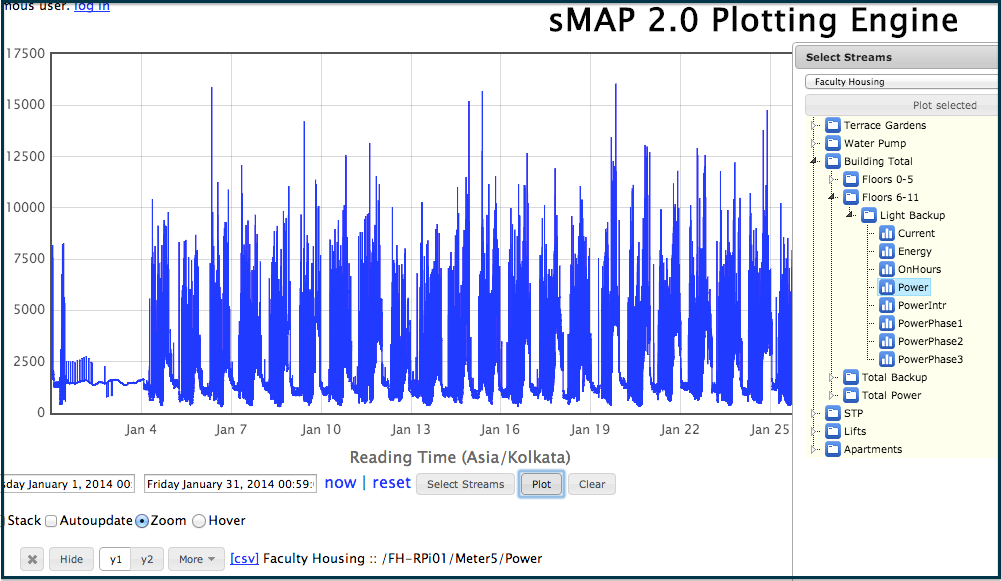
\includegraphics[width=0.8\textwidth,height=0.35\textheight]{screenshot.png}
\caption{Screen shot of the tool that is used to download the energy data of the institute collected over the period of time.}
\label{fig:screenshot}
\end{figure*}


%\item \textbf{ Time Series :} The time series data of the microwave, dryer, kitchen$\_2$ and refrigerator are plotted below in Figures~\ref{fig:micro}, ~\ref{fig:washer}, ~\ref{fig:kitchen2}, ~\ref{fig:refri}.
%
%\begin{figure*}[t]
%\centering
%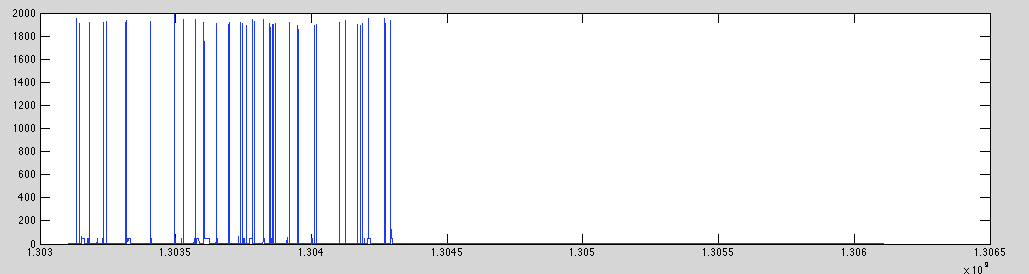
\includegraphics[width=1.0\textwidth,height=0.15\textheight]{channel_6.png}
%\caption{Microwave}
%\label{fig:micro}
%\end{figure*}
%
%\begin{figure*}[t]
%\centering
%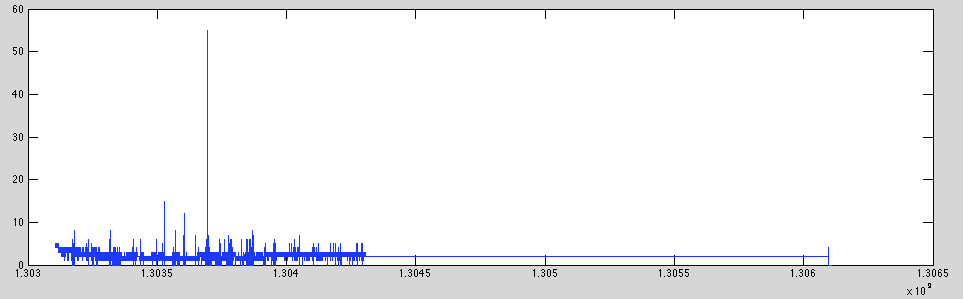
\includegraphics[width=1.0\textwidth,height=0.15\textheight]{channel_7.png}
%\caption{washer\_dryer}
%\label{fig:washer}
%\end{figure*}
%
%\begin{figure*}[th]
%\centering
%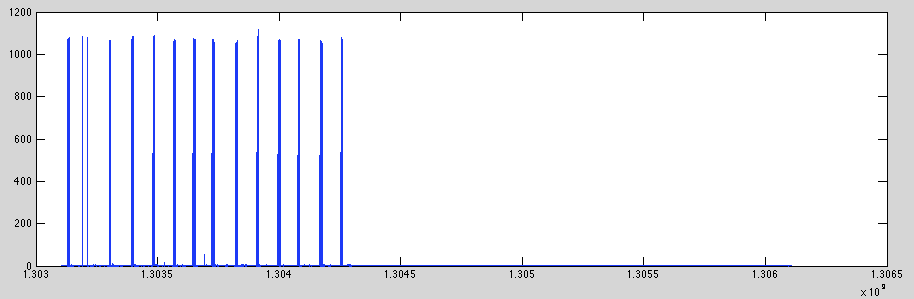
\includegraphics[width=1.0\textwidth,height=0.15\textheight]{channel_8.png}
%\caption{Kitchen\_2}
%\label{fig:kitchen2}
%\end{figure*}
%
%\begin{figure*}[th]
%\centering
%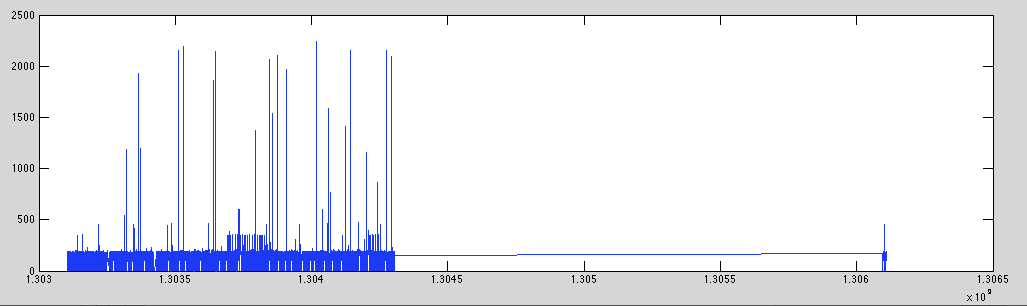
\includegraphics[width=1.0\textwidth,height=0.15\textheight]{channel_9.png}
%\caption{refrigerator}
%\label{fig:refri}
%\end{figure*}
%
%\item \textbf{Code } The implementation of the product of experts model is obtained from Iain Murray's website\footnote{\label{link}http://homepages.inf.ed.ac.uk/imurray2/code/}. It implements the technique described in Geoff Hinton's paper \cite{hinton2000}. 
%
%\item \textbf{Additional details }
%Some additional details regarding experiments:
%\begin{enumerate}
%\item The product of HMMs model (PoHMM) minimizes ``contrastive divergence" as described in the paper \cite{hinton2000}. 
%\item The number of experts, $k$ used here is 15. This is set somewhat arbitrarily and needs to be experimented on.
%\item Learning rate is $\epsilon = \frac{1}{300}$.
%\end{enumerate}
 
\end{itemize}

\subsection{Problem Formulation}
The disparate energy data streams collects readings at different time scales. Each of the data stream is modelled as a HMM with cardinality $2$, that is either ON or OFF. The process of aggregating the energy data from different data streams is modelled through PoHMMs. 

%Different smart meters can send data points when they are collected resulting in inconsistent data including aggregating non-aligned time stamped readings, readings with missing values, repeated values, meter reset readings.
%We address the problem of learning from disparate data streams (with inconsistencies) by modelling streams as HMMs and the process of aggregating data at the base station as a Product of HMMs. This enables us to perform load forecasting using machine learning techniques.
Each energy data stream is used to train the model, till the time the objective function, that is contrastive divergence reaches a threshold value. Once the model is trained from a randomly sampled data stream, the parameters learned by the model %(mixing component of each unigauss, means of gaussian bits, log precisions of axis-aligned gaussian bits) 
are provided to the randomly sampled test set (total energy consumed data) to obtain the conditional probability distribution of the gaussians given the data. Similarly, all the data streams are used for training the model, and the parameters learned are then applied on the test set to obtain the conditional probability of the gaussians given the data. After all the data streams are used to obtain the probability distribution, we use the data stream that correspond to the total energy consumed from the house/ building to train the model and hence obtain the probability distribution P of the gaussians. These probability distributions are then compared with the product of the probability distributions Q obtained from the individual data streams. The evaluation of how well the learning has taken place is done by using a Kullback-Leibler divergence. KL divergence of two probability distributions P and Q, $D_{KL}$(P$\parallel$Q) is the measure of information lost when Q is used to approximate P. %Here, P is the real data and Q is a fantasy data. The two probability distributions in the REDD example refer to the expert probabilities in real and fantasy data. 
%The learned parameters from the training are fitted to the fantasy data to measure the information lost when fantasy data is used to approximate real data.


%\subsection{Experimental Setup}
%%Experiments are performed on the REDD which contains $9$ appliances each containing $318759$ rows of energy consumption data. 
%Experiments are done into $4$ phases, in the first phase the number of data samples are varied corresponding to which the values of KL Divergence and convergence time are noted. In the second phase, the number of experts are varied keeping the best value of the sample from the first phase fixed. In the third phase, number of iterations are varied keeping the best values from above first two phases fixed. In the fourth part, the no. of appliances to be aggregated are varied.

\begin{table*}[htdp]
\begin{center}
\begin{tabular}{| c | c | c | c |}
\hline
Samples & $KL Div$ & $T(sec)$ & $Iterations$ \\
\hline
300 & 2.4864 & 186.212 $\pm$9.087 & 18600 \\
500 & 0.6761 & 106.564 $\pm$10.046 & 10200 \\
1000 & 1.1088 & 158.521 $\pm$1.97  & 11200 \\
1500 & 3.8829 & 92.896 $\pm$8.075  & 5300 \\
2000 & 1.8686 & 130.98 $\pm$1.932 & 6900 \\
2500 & 0.4733 & 215.563 $\pm$ 2.471 & 9900 \\
3000 & 2.8204 & 258.213 $\pm1.918$ & 11000 \\
3500 & 1.2332 & 204.661 $\pm$1.713 & 7900 \\
4000 & 0.8959 & 292.666 $\pm$0.619 & 10400  \\
4500 & 1.1118 & 222.558 $\pm$1.967 & 7200  \\
8000 & 6.392 & 381.635 $\pm$2.952 & 8100  \\
10000 & 8.276 & 887.932 $\pm$13.824 & 10500  \\
15000 & 0.7201 & 1368.514 $\pm$13.605 & 9400  \\
\hline
\end{tabular}
\end{center}
\caption{Effect of varying samples on KL div and time for REDD}
\label{table:sample1}
\end{table*}

%\begin{table}[htdp]
%\begin{center}
%\begin{tabular}{| c | c | c | c |}
%\hline
%Experts & $KL Div$ & $T(sec)$ & $Iterations$ \\
%\hline
%5 & 0.774 & 72.968 $\pm$1.177 & 5200 \\
%10 & 1.424 & 117.482 $\pm$1.966 & 6700 \\
%15 & 0.473 & 210.249 $\pm$1.258  & 9900 \\
%20 & 1.56 & 217.739 $\pm$10.452 & 9000 \\
%25 & 7.469 & 347.019 $\pm$8.23 & 12100 \\
%30 & 2.4968 & 413.802 $\pm$7.304 & 12900 \\
%35 & 1.5012 & 348.906 $\pm$14.651 & 11300 \\
%\hline
%\end{tabular}
%\end{center}
%\caption{Effect of varying experts on KL div and time}
%\label{table:expert}
%\end{table}


\subsection{Empirical Results}
In both the datasets, experiments are performed by tuning some parameters and keeping some fixed. In case of REDD, Tables~\ref{table:sample1},~\ref{table:threshold1} and~\ref{table:appliance1} show the effect of varying data samples, threshold and no. of appliances on the KL divergence.
In case of faculty housing dataset, Tables~\ref{table:sample2} and~\ref{table:expert2} show the effect of varying data samples and no. of HMMs on the KL divergence.

%Experiments are done into $4$ phases, in the first phase the number of data samples are varied corresponding to which the values of KL Divergence and convergence time are noted. In the second phase, the number of experts are varied keeping the best value of the sample from the first phase fixed. In the third phase, number of iterations are varied keeping the best values from above first two phases fixed. In the fourth part, the no. of appliances to be aggregated are varied.

%The evaluation of how well the learning has taken place is done by using a Kullback-Leibler divergence. KL divergence of P from Q, $D_{KL}$(P$\parallel$Q) is the measure of information lost when Q is used to approximate P. Here, P is the real data and Q is a fantasy data. The two probability distributions in the REDD example refer to the expert probabilities in real and fantasy data. The learned parameters from the training are fitted to the fantasy data to measure the information lost when fantasy data is used to approximate real data.


\begin{table*}[htdp]
\parbox{.51\linewidth}{
\centering
\begin{tabular}{| c | c | c | c |}
\hline
Threshold & $KL Div$ & $T(sec)$ & $Iterations$ \\
\hline
.1 & 0.473 & 210.6 $\pm$1.493 & 9900 \\
.05 & 0.443 & 240.607$\pm$2.436 & 10900 \\
.01 & 0.454 & 431.536 $\pm$14.509 & 18000 \\
.005 & 0.509 & 1167.243 $\pm$43.412 & 49800 \\
\hline
\end{tabular}
\caption{Effect of varying min threshold on KL div and time for REDD}
\label{table:threshold1}
}
\hfill
\parbox{.51\linewidth}{
\centering
\begin{tabular}{| c | c | c | c |}
\hline
Appliances & $KL Div$ & $T(sec)$ & $Iterations$ \\
\hline
3 & 5.559 & 233.664 $\pm$0.579 & 10700 \\
4 & 0.188 & 465.634 $\pm$5.275 & 19900 \\
5 & .432 & 338.416 $\pm$3.988  & 13400 \\
6 & 8.736 & 606.062 $\pm$7.534 & 28100 \\
7 & 5.054 & 411.457 $\pm$10.051 & 17300 \\
8 & 0.436 & 260.544 $\pm$27.862 & 10700 \\
9 & 0.15 & 474.579 $\pm$14.619 & 20600 \\
\hline
\end{tabular}
\caption{Effect of varying appliances on KL div and time for REDD}
\label{table:appliance1}
}
\end{table*}


\begin{table*}[htdp]
\parbox{.51\linewidth}{
\centering
\begin{tabular}{| c | c | c | c |}
\hline
Samples & $KL Div$ & $T(sec)$ & $Iterations$ \\
\hline
100 & 2.6219e-05 & 257 & 45100 \\
300 & 1.9753e-05 & 222 & 43200 \\
500 & 5.5493e-05 & 260 & 44800 \\
700 & 3.2847e-05 & 249 & 44000 \\
900 & 3.9486e-04 & 221 & 42600 \\
1100 & 4.9274e-04 & 317 & 44700 \\
1300 & 3.0425e-04 & 276 & 43100 \\
1500 &  3.1128e-04 & 303 & 44400\\
2000 & 1.9192e-04 & 306 & 44400\\
2500 & 1.7122e-04 & 370 & 44100 \\
3000 & 1.4686e-04 & 331 & 43300 \\
3500 & 1.2663e-04 & 370 & 43200 \\
4000 & 1.0793e-04 & 403 & 43200 \\
\hline
\end{tabular}
\caption{Effect of varying samples on KL div for housing data}
\label{table:sample2}
}
\hfill
\parbox{.51\linewidth}{
\centering
\begin{tabular}{| c | c | c |}
\hline
HMMs & $KL Div (e-05)$ & $T(sec)$\\
\hline
2 & 0 & 219 \\
3 & 1.9780 & 229 \\
4 & 3.5897 & 217 \\
5 & 1.9753 & 228 \\
6 & 4.3488 & 238 \\
7 & 4.9111 & 245  \\
8 & 5.6564 & 241 \\
9 & 5.4290 & 258 \\
10 & 5.5163 & 267 \\
12 & 4.4504 & 262 \\
14 & 6.9006 & 296 \\
16 & 6.8666 & 300 \\
18 & 6.2872 & 313 \\
20 & 5.3842 & 267 \\
25 & 5.8970 & 326 \\
30 & 5.9962 & 327  \\
35 & 5.2716 & 346 \\
40 & 5.0955 & 320 \\
\hline
\end{tabular}
\caption{Effect of varying HMMs on KL div and time for housing data}
\label{table:expert2}
}
\end{table*}


\subsection{Discussion}
As per table \ref{table:sample1} and \ref{table:sample2}, the relation between no. of samples and KL divergence was observed, the best performance was attained when $2500$ and $300$ samples were taken from the REDD and faculty housing dataset respectively. Whereas in table \ref{table:threshold1}, there is an indirect relationship of threshold value and KL divergence, that is lower the threshold, higher the KL divergence in contrast to the
 direct relationship between the threshold value and the time taken or the iterations required. Table \ref{table:appliance1} and \ref{table:expert2} show that when all the appliances in the home are used in PoHMMs the performance is at its best. The value of KL divergence is minimum when the energy data from all the appliances are aggregated and tested with total energy data. % keeping the threshold value fixed at $0.1$ and no. of appliances fixed at $15$.

\section{Conclusions}
In this paper, we are solving the problem of load aggregation (energy consumption) for disparate energy data sources using the ensemble based learning technique called Product of HMMs. Several challenges are faced while computing the aggregated energy, few of which include non-aligned timestamp readings, missing values, meter reset readings. This technique produces the combined probability distributions of several simpler distributions and then renormalizes this output. The optimisation problem is to minimise the contrastive divergence between the two probability distributions of the data at time $0$ and the data at time $1$ (one-step reconstruction using gibbs sampling). The evaluation of the algorithm is done by computing the KL divergence between the product of the energy data distributions and the total energy data distribution. From the results shown in table \ref{table:appliance1} and \ref{table:expert2}, we can see that the algorithm has performed best when the number of appliances (REDD) reached the actual number of appliances ($9$) in the house and the number of data streams in case of housing data reached the actual number of streams ($2$) used in the 12 floor faculty housing data. Therefore, this signifies that this algorithm is applicable for this kind of application and can be used for load forecasting.


\label{sec:con}

% An example of a floating figure using the graphicx package.
% Note that \label must occur AFTER (or within) \caption.
% For figures, \caption should occur after the \includegraphics.
% Note that IEEEtran v1.7 and later has special internal code that
% is designed to preserve the operation of \label within \caption
% even when the captionsoff option is in effect. However, because
% of issues like this, it may be the safest practice to put all your
% \label just after \caption rather than within \caption{}.
%
% Reminder: the "draftcls" or "draftclsnofoot", not "draft", class
% option should be used if it is desired that the figures are to be
% displayed while in draft mode.
%
%\begin{figure}[!t]
%\centering
%\includegraphics[width=2.5in]{myfigure}
% where an .eps filename suffix will be assumed under latex, 
% and a .pdf suffix will be assumed for pdflatex; or what has been declared
% via \DeclareGraphicsExtensions.
%\caption{Simulation Results}
%\label{fig_sim}
%\end{figure}

% Note that IEEE typically puts floats only at the top, even when this
% results in a large percentage of a column being occupied by floats.


% An example of a double column floating figure using two subfigures.
% (The subfig.sty package must be loaded for this to work.)
% The subfigure \label commands are set within each subfloat command, the
% \label for the overall figure must come after \caption.
% \hfil must be used as a separator to get equal spacing.
% The subfigure.sty package works much the same way, except \subfigure is
% used instead of \subfloat.
%
%\begin{figure*}[!t]
%\centerline{\subfloat[Case I]\includegraphics[width=2.5in]{subfigcase1}%
%\label{fig_first_case}}
%\hfil
%\subfloat[Case II]{\includegraphics[width=2.5in]{subfigcase2}%
%\label{fig_second_case}}}
%\caption{Simulation results}
%\label{fig_sim}
%\end{figure*}
%
% Note that often IEEE papers with subfigures do not employ subfigure
% captions (using the optional argument to \subfloat), but instead will
% reference/describe all of them (a), (b), etc., within the main caption.


% An example of a floating table. Note that, for IEEE style tables, the 
% \caption command should come BEFORE the table. Table text will default to
% \footnotesize as IEEE normally uses this smaller font for tables.
% The \label must come after \caption as always.
%
%\begin{table}[!t]
%% increase table row spacing, adjust to taste
%\renewcommand{\arraystretch}{1.3}
% if using array.sty, it might be a good idea to tweak the value of
% \extrarowheight as needed to properly center the text within the cells
%\caption{An Example of a Table}
%\label{table_example}
%\centering
%% Some packages, such as MDW tools, offer better commands for making tables
%% than the plain LaTeX2e tabular which is used here.
%\begin{tabular}{|c||c|}
%\hline
%One & Two\\
%\hline
%Three & Four\\
%\hline
%\end{tabular}
%\end{table}


% Note that IEEE does not put floats in the very first column - or typically
% anywhere on the first page for that matter. Also, in-text middle ("here")
% positioning is not used. Most IEEE journals/conferences use top floats
% exclusively. Note that, LaTeX2e, unlike IEEE journals/conferences, places
% footnotes above bottom floats. This can be corrected via the \fnbelowfloat
% command of the stfloats package.




% conference papers do not normally have an appendix


% use section* for acknowledgement

%\section*{Acknowledgment}
%
%
%The authors would like to thank...



\nocite{Rabiner,SS97a,Kawamoto,Diane,Klopfert,Ghahramani,Felice,Shen,taban,Albert,wijaya2014consumer,Zhang,Daneshi,bassi,samuel,Falvo,Bakirtzis,Chen,Chow,DisaggregationHSMM,KolterJ12,KolterF11,BLTJ:BLTJ21650,Heinzelman00energy,Taylor,NYAS:NYAS5921,
Wijaya,5620917,1626400,mckerracher,hinton2000,aistats,fhmm,andrew}

% trigger a \newpage just before the given reference
% number - used to balance the columns on the last page
% adjust value as needed - may need to be readjusted if
% the document is modified later
%\IEEEtriggeratref{8}
% The "triggered" command can be changed if desired:
%\IEEEtriggercmd{\enlargethispage{-5in}}

% references section

% can use a bibliography generated by BibTeX as a .bbl file
% BibTeX documentation can be easily obtained at:
% http://www.ctan.org/tex-archive/biblio/bibtex/contrib/doc/
% The IEEEtran BibTeX style support page is at:
% http://www.michaelshell.org/tex/ieeetran/bibtex/
\bibliographystyle{IEEEtran}
% argument is your BibTeX string definitions and bibliography database(s)
%\bibliography{IEEEabrv,IEEEexample}
\bibliography{bare_conf}

% <OR> manually copy in the resultant .bbl file
% set second argument of \begin to the number of references
% (used to reserve space for the reference number labels box)



%\begin{thebibliography}{1}
%
%\bibitem{IEEEhowto:kopka}
%H.~Kopka and P.~W. Daly, \emph{A Guide to \LaTeX}, 3rd~ed.\hskip 1em plus
%  0.5em minus 0.4em\relax Harlow, England: Addison-Wesley, 1999.
%
%\end{thebibliography}
%\bibliographystyle{IEEEtran}
%\bibliography{./IEEEabrv,./IEEEexample}
%\bibliography{IEEEexample}


% that's all folks
\end{document}


